\section{Prostate Cancer}\label{section:intro:prostatecancer}

\subsection{Anatomy}\label{subsection:intro:prostatecancer:anatomy}

The prostate is an exocrine gland of the male reproductive system and possesses an inverted pyramidal form. Its mensurations are usually about 3 centimetres in height by 2.5 centimetres in depth. Its weight is estimated between 15 and 25 grams for an adult. The size of the prostate increases at two moments during development: initially at puberty to reach its normal size then after 60 years of age leading to benign prostatic hyperplasia (BPH \g).

\begin{figure}
	\centering
	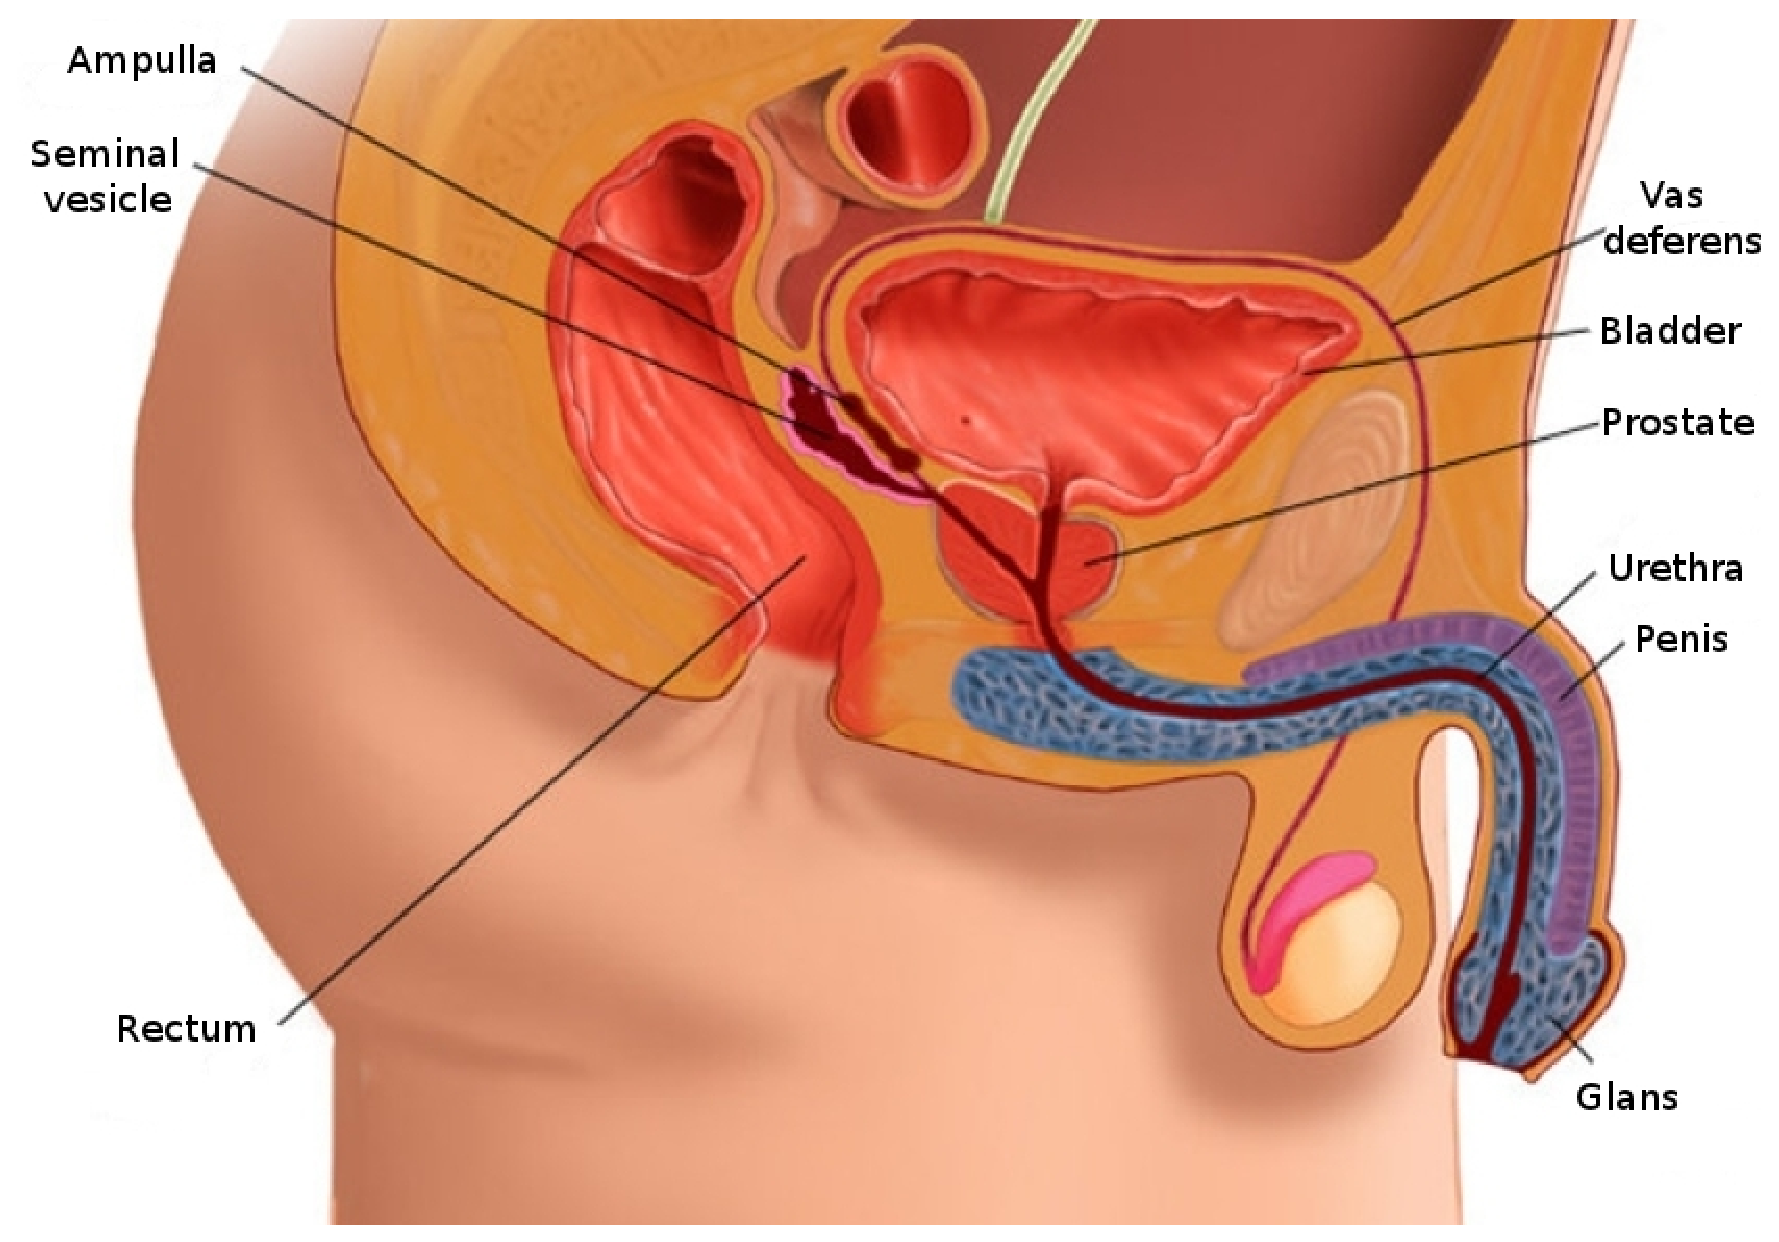
\includegraphics[width=0.65\textwidth]{anatomy/prostate2D.eps}
	\caption{Sagittal anatomy scheme of the male reproductive system \cite{Geckomedia2011}.}
	\label{fig:intro:prostatecancer:anatomy:anatomyProstate2D}
\end{figure}

The prostate is located below the bladder and in the front of the rectum and the urethra goes through the prostate as shown on Fig. \ref{fig:intro:prostatecancer:anatomy:anatomyProstate2D}. The urethral sphincter is located at the apex of the prostate around the prostatic urethra in order to drain the glands. The prostate is also composed of a muscle which allows the expulsion of the sperm during the ejaculation.

\begin{figure}
	\centering
	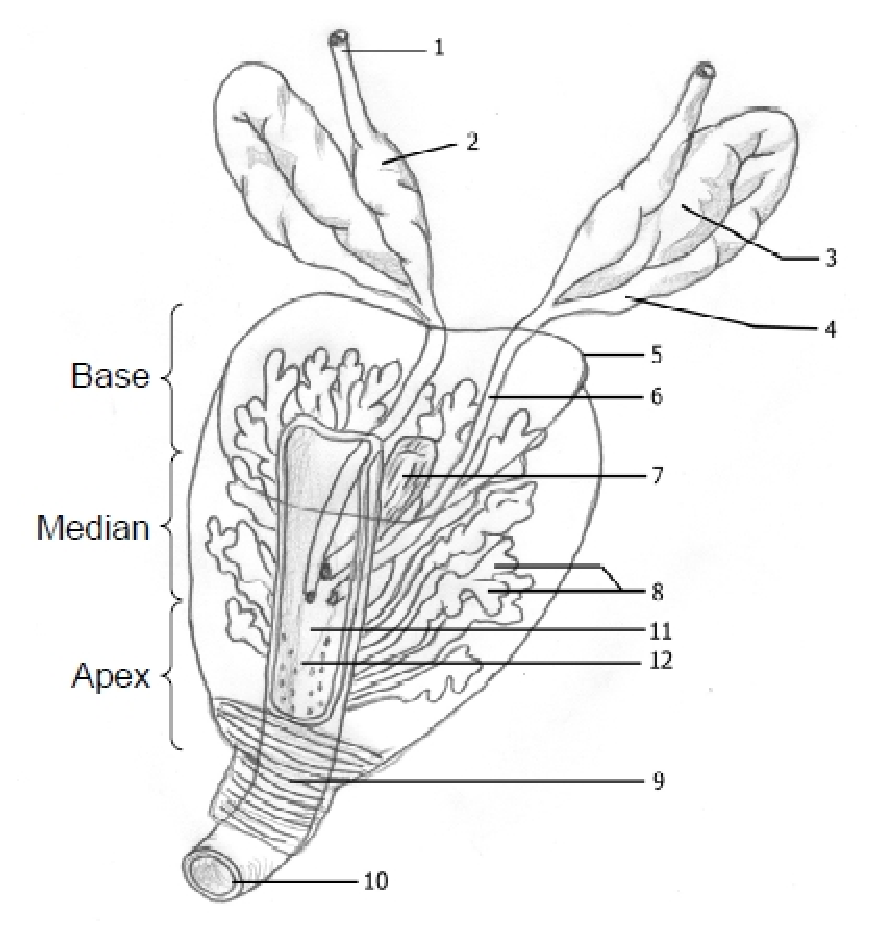
\includegraphics[width=0.50\textwidth]{anatomy/prostate2D2.eps}
	\caption{Representation of the prostate. 1: Vas deferens, 2: Ampulla, 3: Seminal vesicle, 4: Excretory duct of seminal vesicle, 5: Prostate contour, 6: Ejaculatory duct, 7: Prostatic urticle, 8: Glandular tissue, 9: Urethral sphincter, 10: Urethra, 11: Seminal colliculus, 12: Urethral crest \cite{Wikipedia2011}.}
	\label{fig:intro:prostatecancer:anatomy:anatomyProstate2D2}
\end{figure}

The prostate has an inverted pyramidal form. The base is the upper part and closest to the bladder while the apex is lower down and further from the bladder (Fig. \ref{fig:intro:prostatecancer:anatomy:anatomyProstate2D} and \ref{fig:intro:prostatecancer:anatomy:anatomyProstate2D2}). The seminal vesicles are located above the base of the prostate localized between the rectum and the bladder (Fig. \ref{fig:intro:prostatecancer:anatomy:anatomyProstate2D}).

\begin{figure}
	\centering
	\subfigure[Transverse anatomy of the prostate.]{
			\centering
			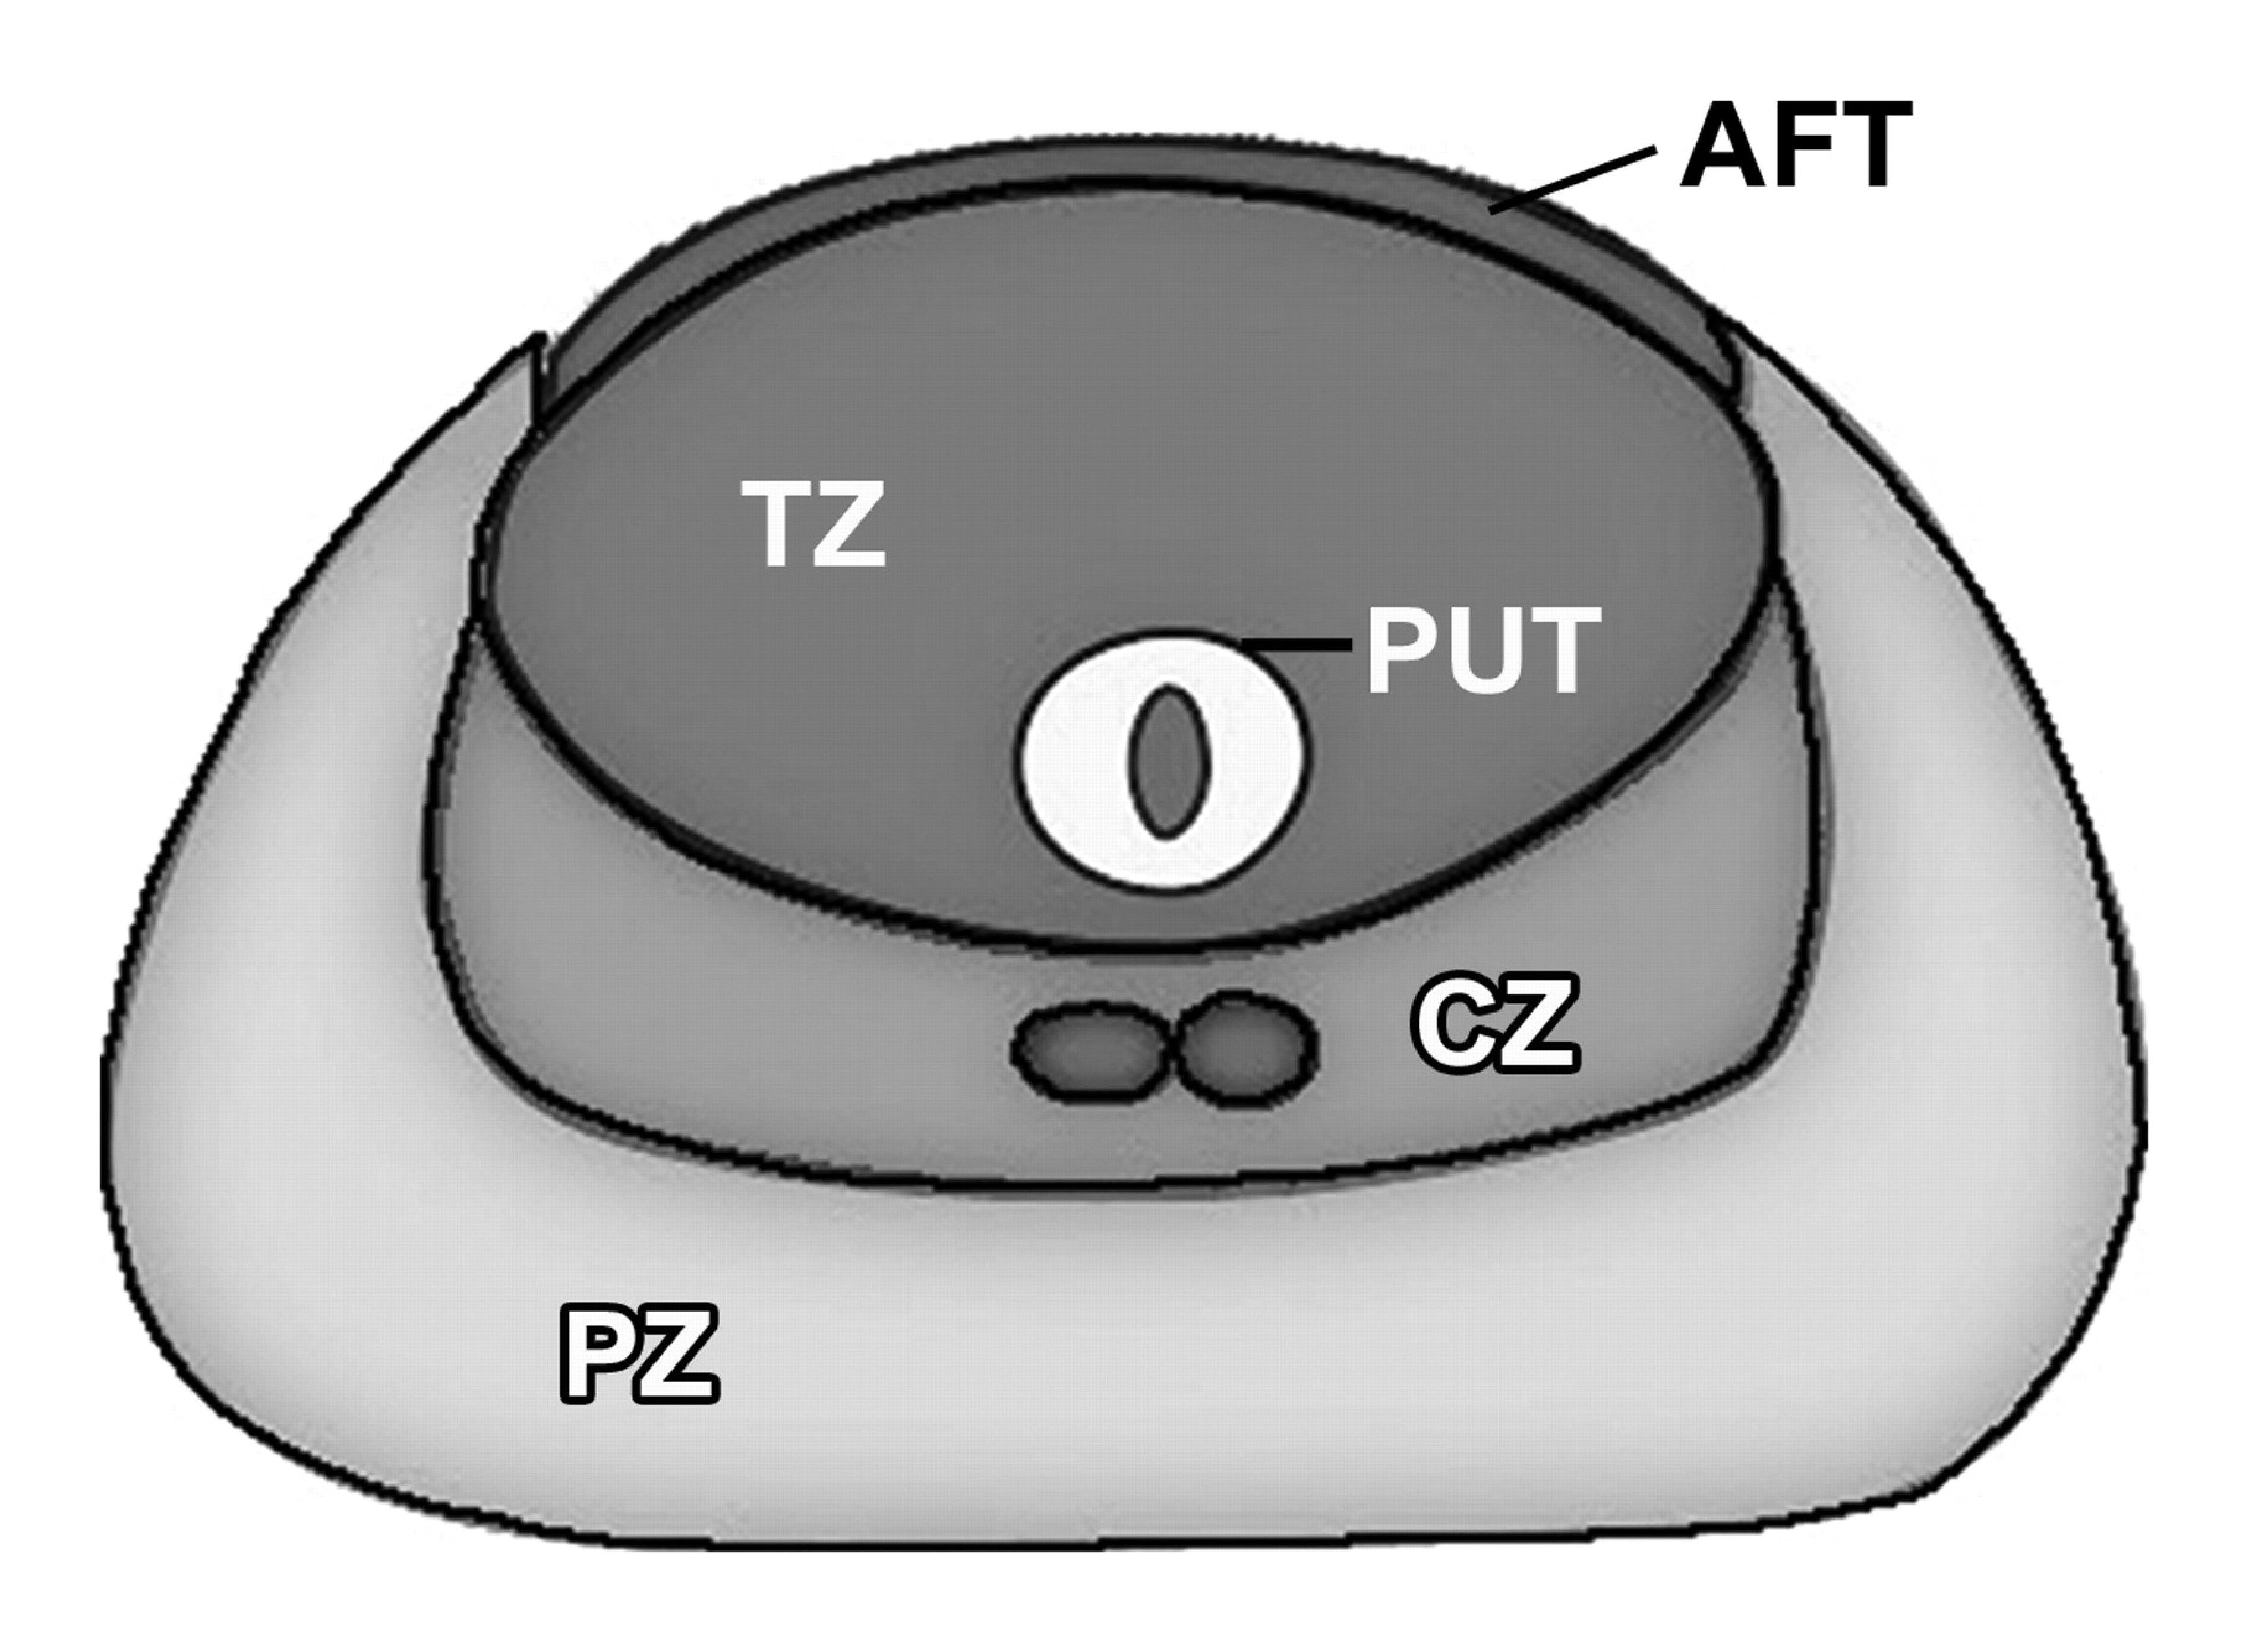
\includegraphics[width=0.4\textwidth]{anatomy/prostateTransverse.eps}
			\label{fig:anatomyProstateTransverse}}
	~~~
	\subfigure[Sagital anatomy of the prostate.]{
			\centering
			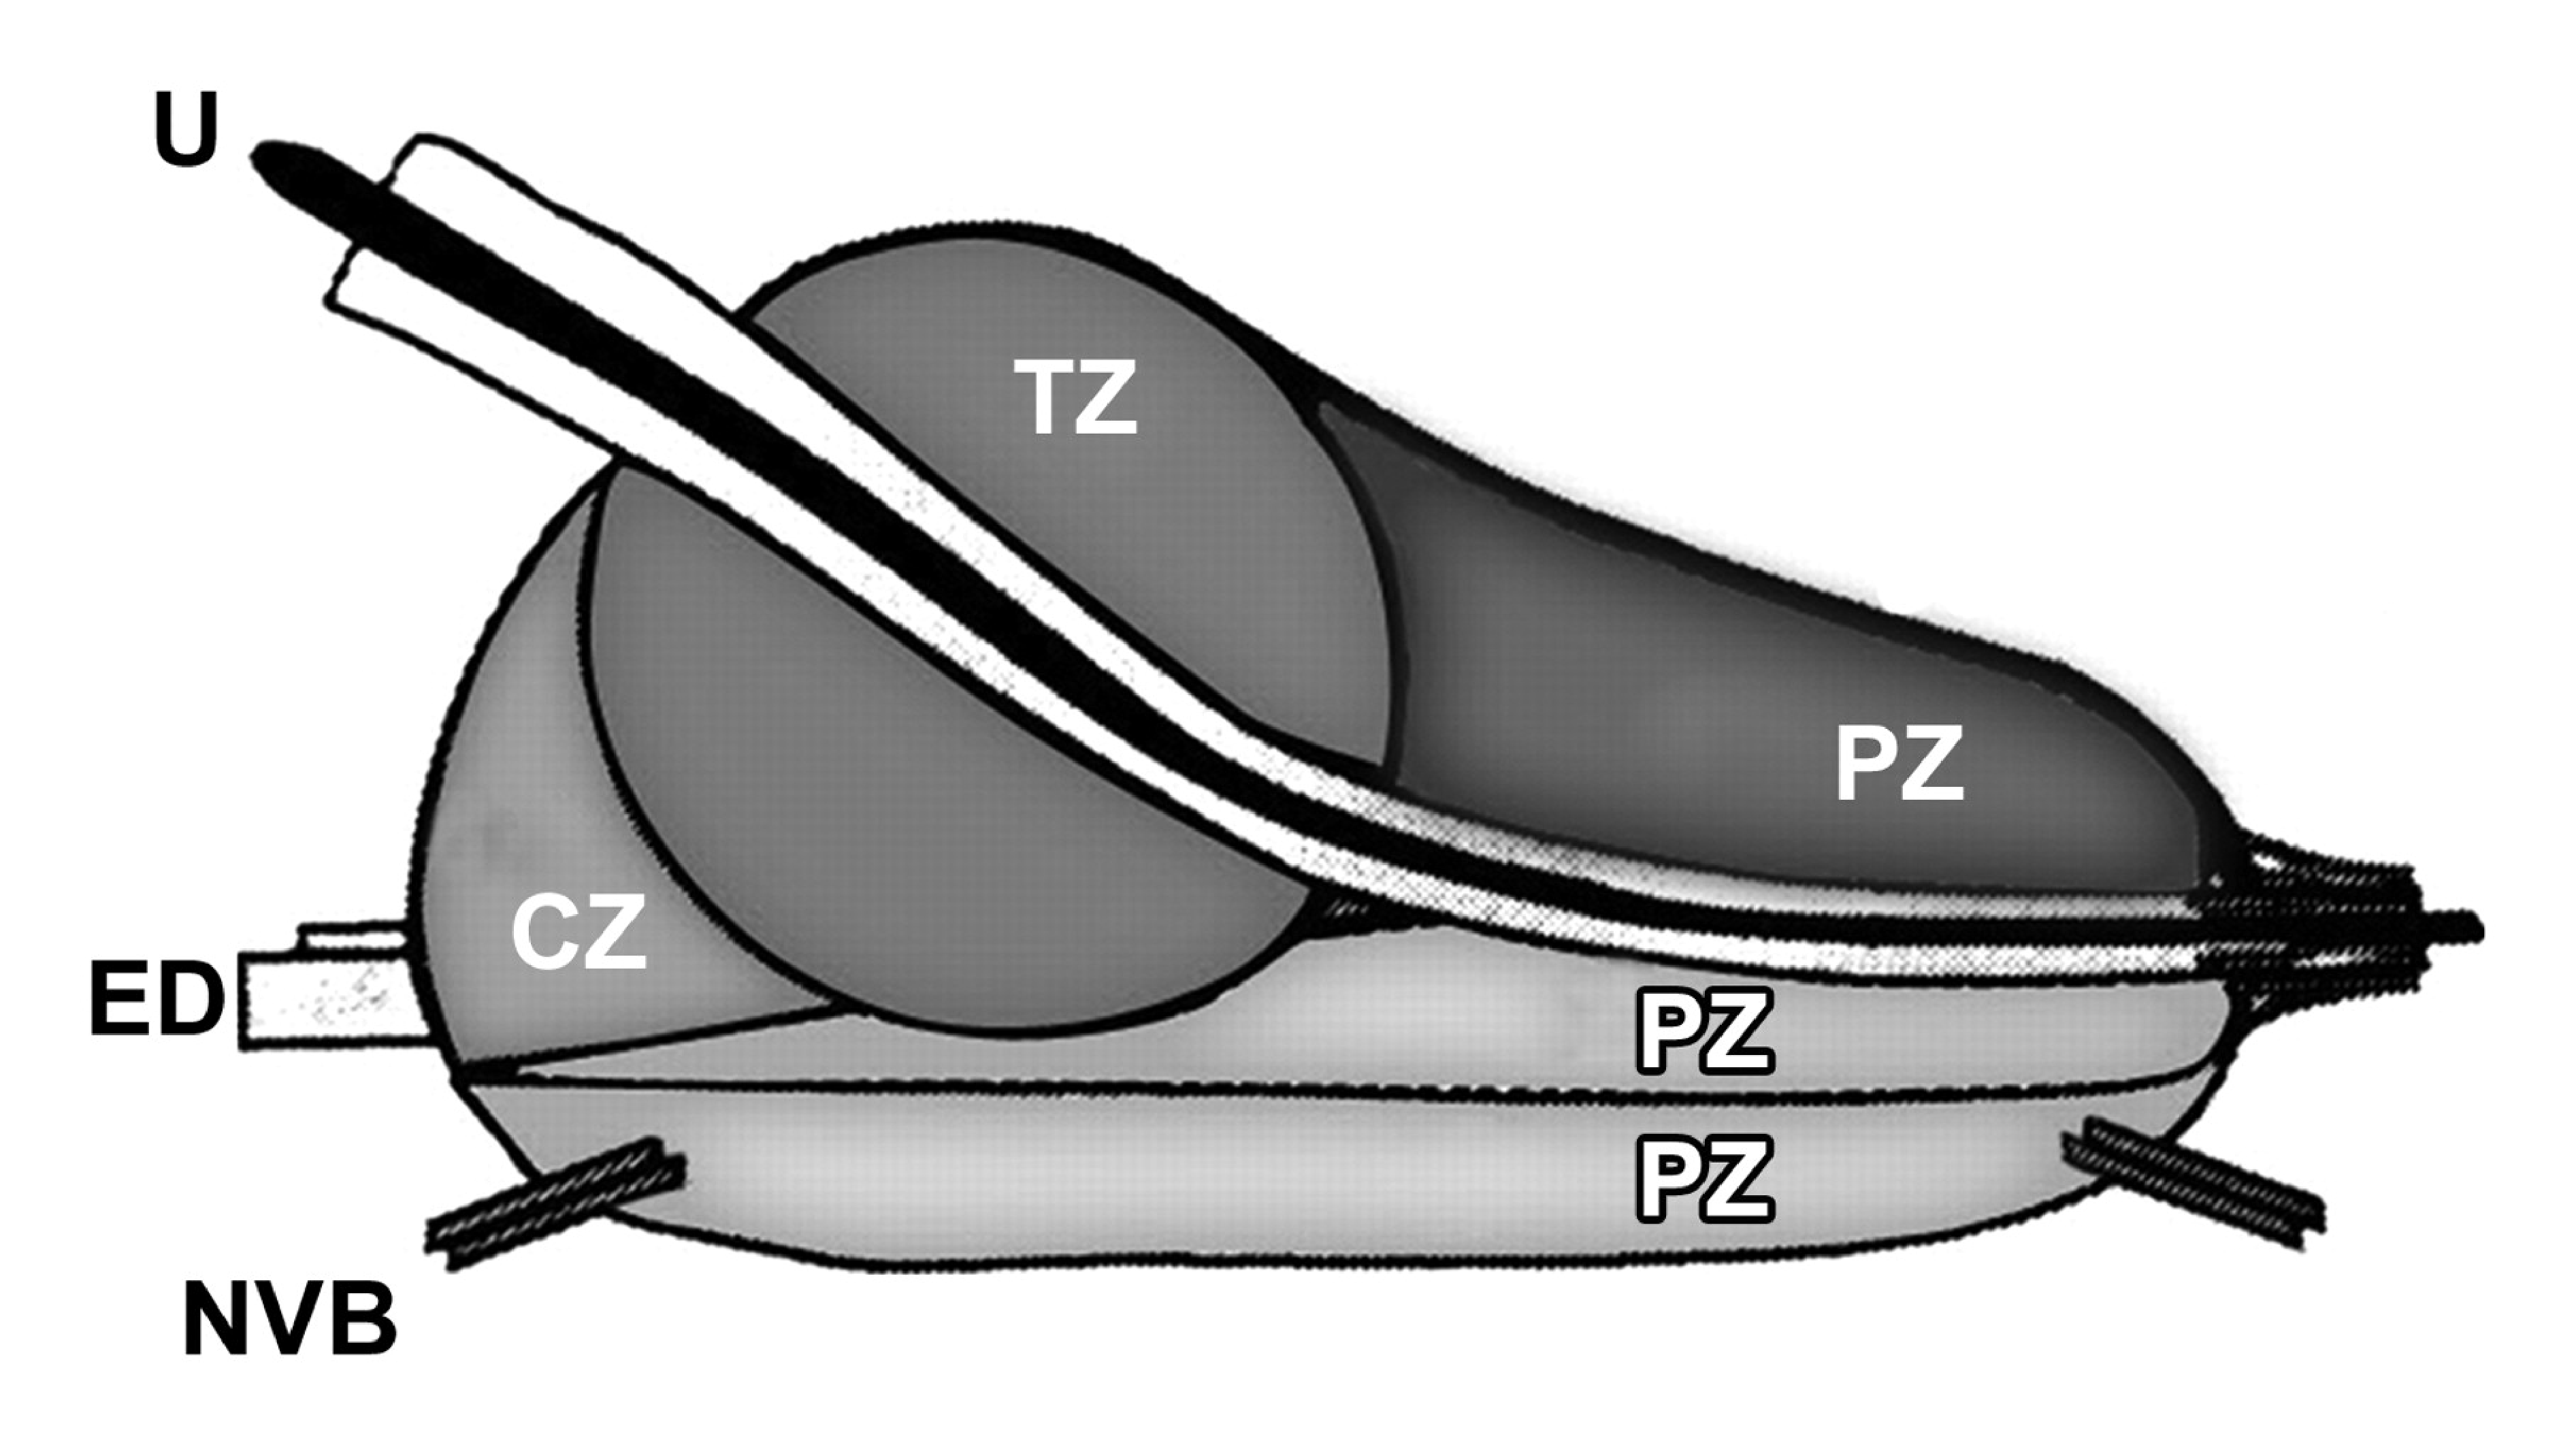
\includegraphics[width=0.4\textwidth]{anatomy/prostateSagital.eps}
			\label{fig:anatomyProstateSagital}}
	\caption{Presentation of the different zones of the prostate. \textit{AFT:} anterior fibromuscular tissue, \textit{CZ:} central zone, \textit{ED:} ejaculatory duct, \textit{NVB:} neurovascular bundle, \textit{PUT:} periurethral tissue, \textit{PZ:} peripherical zone, \textit{U:} urethra, \textit{TZ:} transitional zone \cite{Choi2007}.}
	\label{fig:intro:prostatecancer:anatomy:anatomyProstateZone}
\end{figure}

The prostate can be divided in different zones (Fig. \ref{fig:intro:prostatecancer:anatomy:anatomyProstateZone}) as proposed by McNeal \cite{McNeal1981} and widely accepted in the literature \cite{Hricak1987,Villers1991,Coakley2000,Parfait2010}: central zone (CZ\g), transitional zone (TZ\g) and peripheral zone (PZ\g).

The PZ which represents about 70\% of the prostate is composed of glandular tissue. Roughly 70\% of prostate cancers (PCa\g) originate in this zone.

The CZ which accounts for about 20-25\% of the prostate is composed of stromal tissue. The excretory ducts of the seminal vesicles and ampulla go through the base and join to form the ejaculatory duct.

The TZ is composed of two symmetric lobes localized on each sides of the urethra. The TZ represents 5\% of the prostate. The size of this zone increases with age and with the development of a pathology known as benign prostatic hyperplasia.

Approximately 30\% of PCa are found in these two zones.

On MRI images, the CZ and TZ are usually difficult to distinguish.

The PZ accounts for about 70\% of glandular tissue. 70\% of PCa arise in this zone.

\subsection{Statistics}\label{subsection:intro:prostatecancer:statistics}

\subsubsection{Overview}\label{subsubsection:intro:prostatecancer:statistics:overview}

The World Health Organization (WHO) published in 2008 that PCa was the second most frequently diagnosed cancer of men and the fifth most common cancer overall \cite{Ferlay2010}. No less than 899,000 new cases where detected worldwide in 2008 \cite{Ferlay2010}. As presented on Fig. \ref{fig:intro:prostatecancer:statistics:overview:repartitionCancer}, PCa accounts for approximately 7.1\% (Fig. \ref{fig:intro:prostatecancer:statistics:overview:repartitionCancerIncidence}) of all cancers diagnosed in 2008 and 3.4\% (Fig. \ref{fig:intro:prostatecancer:statistics:overview:repartitionCancerDeaths}) of all cancers deaths in 2008 \cite{Ferlay2010}.

\begin{figure}
	\centering
	\subfigure[Estimated number cancers cases for both sexes and all ages.]{
			\centering
			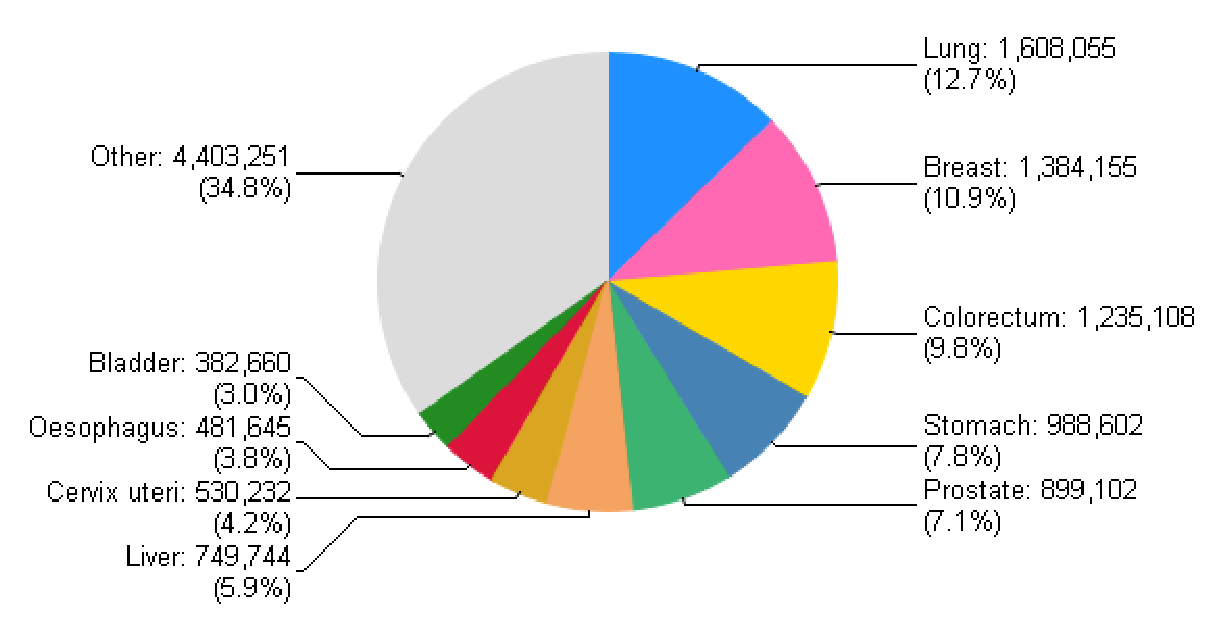
\includegraphics[width=0.65\textwidth]{statistics/repartitionCancerIncidence.eps}
			\label{fig:intro:prostatecancer:statistics:overview:repartitionCancerIncidence}}
	~
	\subfigure[Estimated number cancers deaths for both sexes and all ages.]{
			\centering
			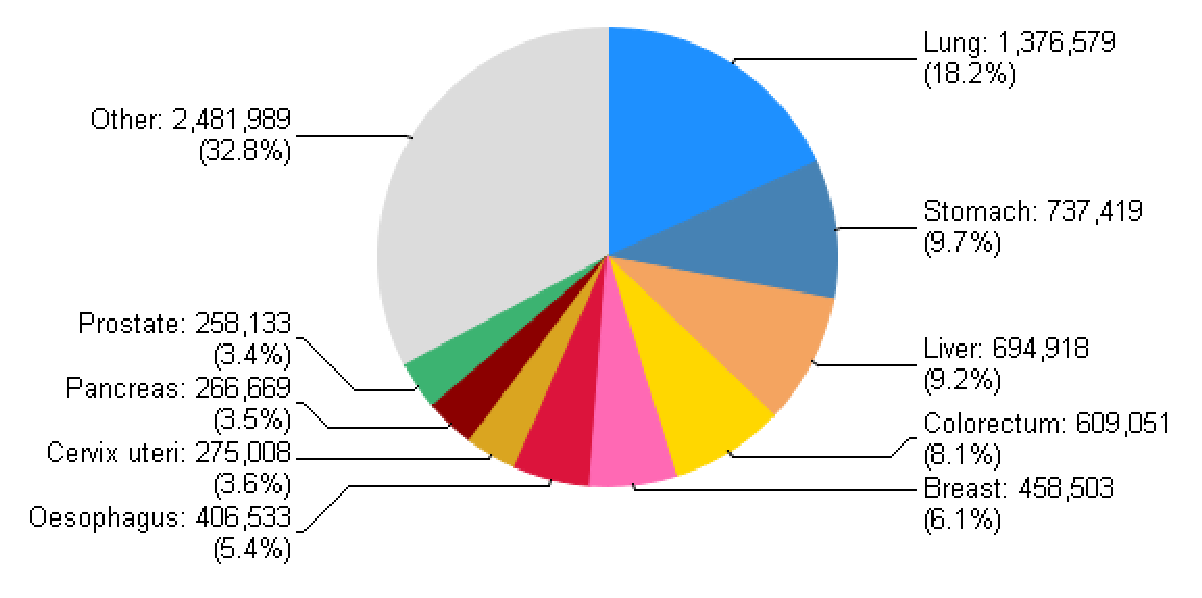
\includegraphics[width=0.65\textwidth]{statistics/repartitionCancerDeaths.eps}
			\label{fig:intro:prostatecancer:statistics:overview:repartitionCancerDeaths}}
	\caption{Cancer estimations in 2008 by the World Health Organization (WHO) \cite{Ferlay2010}.}
	\label{fig:intro:prostatecancer:statistics:overview:repartitionCancer}
\end{figure}

\subsubsection{Risk Factors}\label{subsubsection:intro:prostatecancer:statistics:riskfactors}

The risk factors can be categorized in three different classes: 

\begin{itemize}
	\item Age: age is the most important risk factor for PCa. The diagnosis of PCa for men over 50 years old. PCa rate increases upto about 70 and declines thereafter \cite{AmericanCancerSociety2010}.
	\item Genetic factors: it has been shown that the probability to have a cancer is higher when a member of the family has been already diagnosed \cite{AmericanCancerSociety2010}.
	\item Race: in the United States, the Africo Americans have a higher probability of developing a PCa than European American and Hispanic men \cite{AmericanCancerSociety2010}.
\end{itemize}

\subsection{Diagnosis and Medical Exams}\label{subsubsection:intro:prostatecancer:diagnosis}

The presence of PCa may be suggested in several ways: digital rectal examination, Prostate Specific Antigen (PSA\g) test, biopsy using transrectal ultrasound (TRUS\g) and magnetic resonance imaging (MRI\g-MRSI\g).

\subsubsection{Digital Rectal Examination}\label{subsubsection:intro:prostatecancer:diagnosis:rectalexamination}

Both benign prostatic hyperplasia and cancer may lead to an increasing size of the prostate. A rectal examination may allow detection of harder nodules within the softer prostatic tissue. The advantages are that this method is very fast and does not need any special equipment.

\subsubsection{PSA test}\label{subsubsection:intro:prostatecancer:diagnosis:psa}

The PSA is a protein secreted by the prostate. A higher-than-normal level of PSA can indicate an abnormality of the prostate: a benign prostatic hyperplasia or a cancer. However, other factors can lead to an increasing level of PSA such as prostate infections, irritations, a recent ejaculation or a recent rectal examination, etc.

The PSA can be found in the blood in two different forms: free PSA (about 10\%) and linked to another protein (about 90\%).

A level of PSA higher than 10 $ng.mL^{-1}$ is considered as pathologic \cite{Parfait2010}. If the PSA level is between 10 $ng.mL^{-1}$ and 4 $ng.mL^{-1}$, the patient is considered as suspicious \cite{Parfait2010}. In that case, the ratio free PSA over total PSA is computed. If the ratio is higher than 15\%, the case is considered as pathologic.

\subsubsection{TRUS}\label{subsubsection:intro:prostatecancer:diagnosis:trus}

As described in Sect. \ref{subsection:intro:prostatecancer:anatomy}, the prostate is localized in front of the rectum. Hence, its position allows one to carry out a biopsy using transrectal ultrasound (TRUS) in order to localise more precisely an eventual cancer (Fig. \ref{fig:intro:prostatecancer:diagnosis:trus}).

\textbf{\textit{\textsc{Add example of images of TRUS PCa and not}}}
\begin{figure}
	\centering
	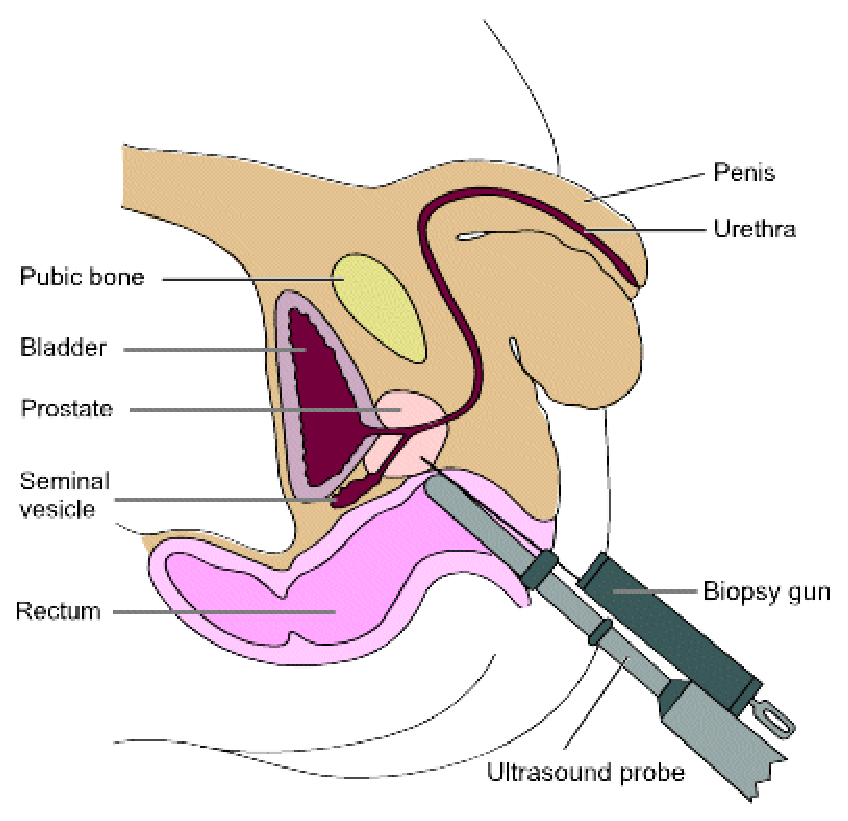
\includegraphics[width=0.45\textwidth]{diagnosis/trus/trus.eps}
	\caption{Biopsy of the prostate using TRUS}
	\label{fig:intro:prostatecancer:diagnosis:trus}
\end{figure}

\textbf{\textit{\textsc{Add information about protocol: manipulation of the patients, which equipment (see Jhimli thesis)}}}
The biopsy is usually prescribed when the PSA level is higher-than-normal or abnormalities were detected during a rectal examination. At least six different samples are taken from the right and left parts of the three different zones: apex, median and base. The samples are analysed in order to determine the presence of a cancer.
\textbf{\textit{\textsc{Add more information on the specificities and accuracy of the techniques. Add also what are the advantages (real-time)}}}

\subsubsection{MRI}\label{subsubsection:intro:prostatecancer:diagnosis:mri}

MRI is a relatively recent technique. This exam allows one to obtain a better spatial resolution and a more precise localization and aggressiveness of the cancer compared with the previous methods. We refer the reader to Sect. \ref{section:intro:mriprinciples} in order to have complete explanation of the different MRI modalities.

The MRI modalities used in PCa diagnosis are: (i) T2-weighted imaging, (ii) diffusion-weighted imaging (DWI\g), (iii) dynamic contrast-enhanced imaging (DCE\g) and (iv) magnetic resonance spectroscopy imaging (MRSI\g).

%\begin{itemize}

%	\item T2-Weighted Imaging:	
%	\begin{figure}
%	\centering
%	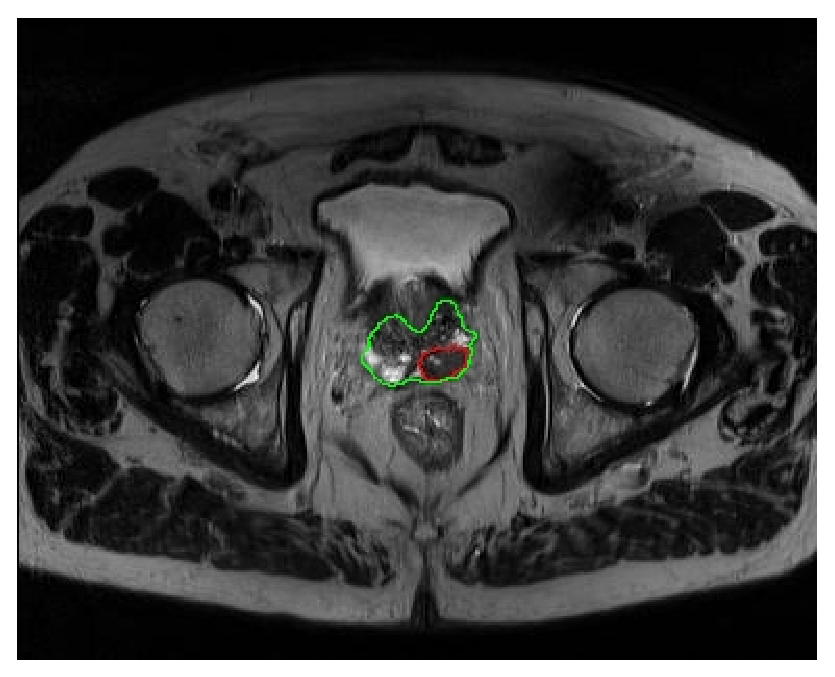
\includegraphics[width=0.45\textwidth]{diagnosis/mri/T2weighted.eps}
%	\caption{T2-Weighted Imaging. The prostate is highlighted in green. The cancer is highlighted in red. Cancer tissue is characterized by a very low-signal intensity allowing to distinguished it easily in the PZ.}
%	\label{fig:intro:prostatecancer:diagnosis:mri:t2weighted}
%	\end{figure}
%T2-weighted imaging provides a spontaneously high contrast image and a good spatial resolution (Fig. \ref{fig:intro:prostatecancer:diagnosis:mri:t2weighted}) depicting precisely the prostate anatomy. Fat, muscles and prostate can easily be differentiated through the contrast between each tissue. The PZ is mainly glandular, which implies a high-signal intensity enclosed by a thin border of low-signal intensity \cite{Carroll2006}. The CZ and TZ are fibrous zones and give a lower signal than that of the PZ \cite{Carroll2006}. Tumours are characterized by very low signal intensity \cite{Carroll2006} implying an easily distinction in PZ. However, note that low signal intensity can be also characteristic of different benign conditions such as haemorrhage, prostatitis, hyperplastic nodules or post-treatment relapses \cite{Claus2004}.

%	\item Diffusion-Weighted Imaging:
%	\begin{figure}
%	\centering
%	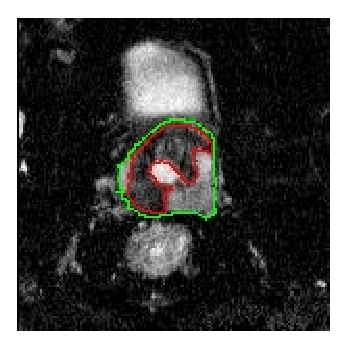
\includegraphics[width=0.45\textwidth]{diagnosis/mri/diffusion.eps}
%	\caption{Diffusion-Weighted Imaging. The prostate is highlighted in green. The cancer is highlighted in red.}
%	\label{fig:intro:prostatecancer:diagnosis:mri:diffusion}
%	\end{figure}
%Diffusion-weighted imaging (DWI\g) represents the degree of diffusion of the water molecules inside the tissue. On DWI images, the prostate can be divided in two parts. The glandular nature of the prostate zone means that tissue. Water is able to move freely and gives a hyper intense signal. The CZ is more chaotic and inhibits the motion of the water. Thus, the signal of CZ will be lower and more heterogeneous than that of the PZ. Tumours imply a greater density of membranes. These membranes also inhibit water motion. Hence, cancer tissue will appear to be darker on DWI images as shown on Fig. \ref{fig:intro:prostatecancer:diagnosis:mri:diffusion}.

%	\item Dynamic Contrast-Enhanced MR Imaging: 
%	\begin{figure}
%	\centering
%	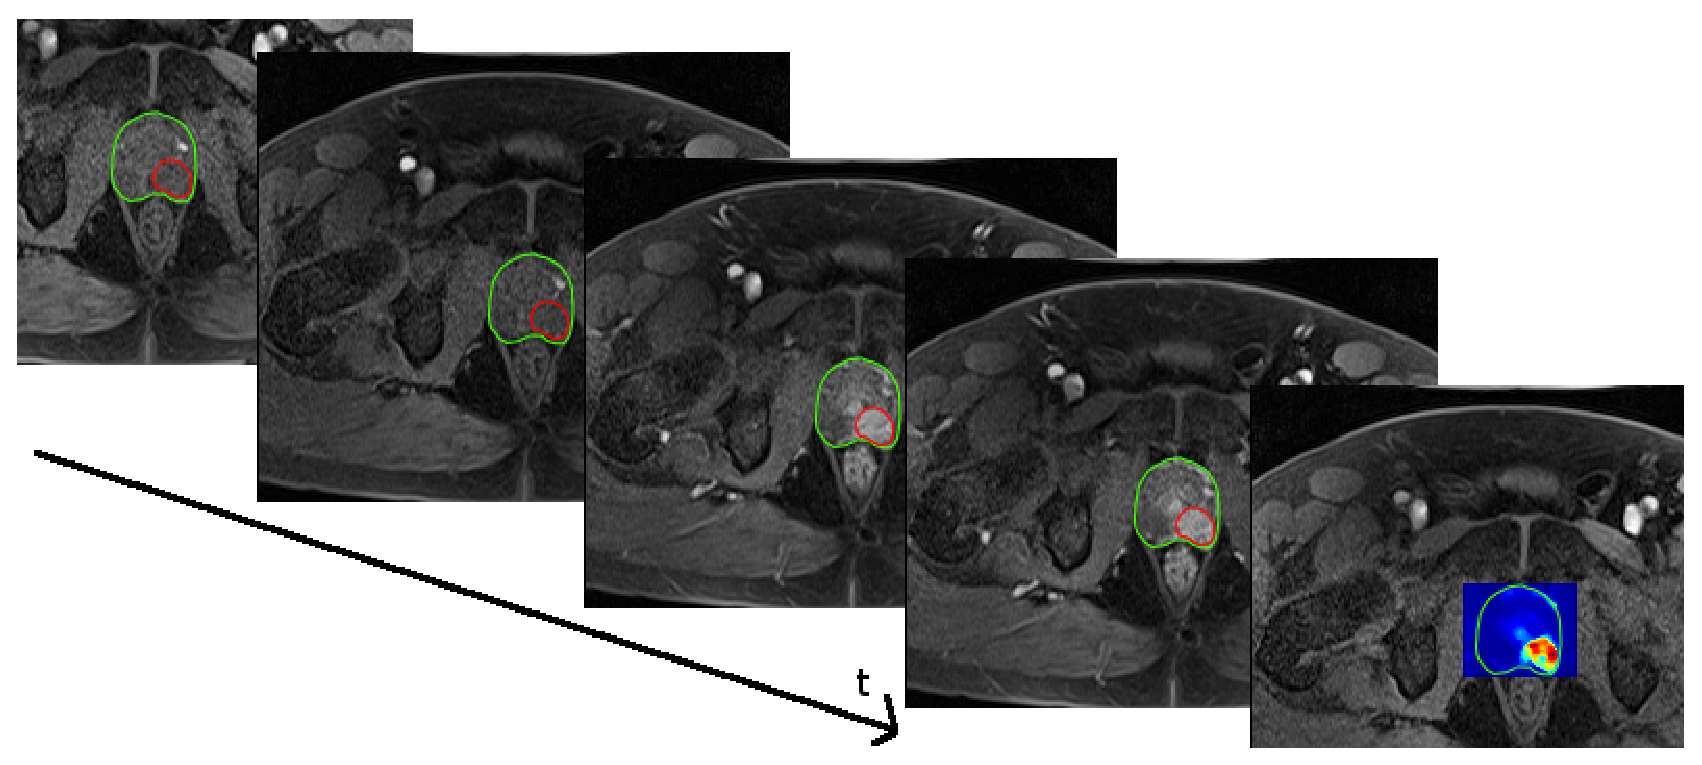
\includegraphics[width=1\textwidth]{diagnosis/mri/perfusion.eps}
%	\caption{Dynamic Contrast-Enhanced MR Imaging. The prostate is highlighted in green. The cancer is highlighted in red. The image contrast changes over time will be studied in order to create a cancer map image (bottom right image).}
%	\label{fig:intro:prostatecancer:diagnosis:mri:perfusion}
%	\end{figure}
%Dynamic contrast-enhanced MR imaging (DCE\g) provides a cinetic study. This technique consists to acquire a series of images in both space and time during the passage of contrast agent (Fig. \ref{fig:intro:prostatecancer:diagnosis:mri:perfusion}). The arrival and departure of the contrast agent will be studied in order to determine the type of tissue. The PZ being mainly composed of glandular tissue the amount of interstitial space is limited involving restricted exchanges and a limited abundance of contrast agent. The signal over time neither rise quickly nor fall off quickly. The CZ has a more disorganised structure which allows easily the arrival of contrast agent. The signal intensity over time will have a rapid increase followed by a plateau. Tumours, due of a high vascularity, will have high exchange in input and in output. Thus, the signal observed during time will have a rapid increase and rapid fall.

%	\item Magnetic resonance spectroscopic imaging:
%	\begin{figure}
%	\centering
%	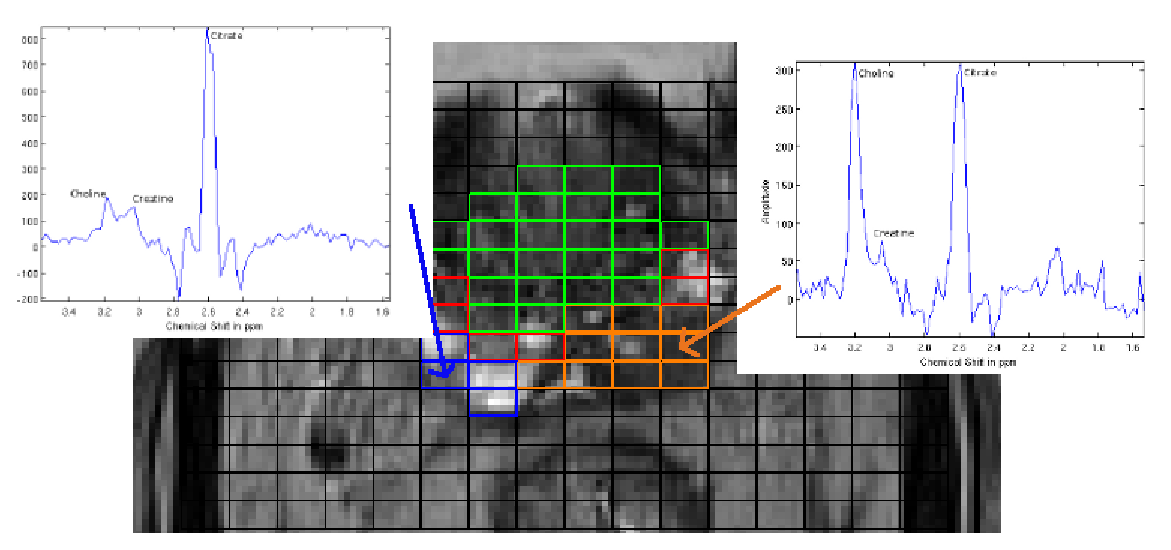
\includegraphics[width=.8\textwidth]{diagnosis/mri/spectro.eps}
%	\caption{MR Spectroscopic Imaging. The prostate voxels are highlighted in color: (i) green - CZ ; (ii) red - TZ ; (iii) blue - PZ ; (iv) orange - PCa. Examples of healthy tissue spectrum (left) and cancer tissue spectrum (right) are given.}
%	\label{fig:intro:prostatecancer:diagnosis:mri:spectro}
%	\end{figure}
%MRSI is a technique that allows the study of metabolite concentrations. The difference in metabolism between healthy and cancer tissues allows one to find a pattern in the concentrations observed. The resolution of the spectroscopy is inferior to the other techniques (Fig. \ref{fig:intro:prostatecancer:diagnosis:mri:spectro}) but this technique is particularly sensitive and bring some information about the aggressiveness of the PCa.
%\end{itemize}